\documentclass[tikz,border=3pt]{standalone}
\usepackage{amsmath,amssymb}
\usetikzlibrary{arrows.meta,positioning,fit,calc,backgrounds,decorations.pathreplacing}

\definecolor{cTeacher}{HTML}{6C5CE7}
\definecolor{cSlow}{HTML}{2878B5}
\definecolor{cFast}{HTML}{E67E22}
\definecolor{cInk}{HTML}{263238}

\tikzset{
  flow/.style={-{Latex[length=2.0mm]},line width=0.7pt,draw=cInk!75},
  dashflow/.style={-{Latex[length=2.0mm]},line width=0.65pt,draw=cInk!55,dashed},
  plain/.style={line width=0.7pt,draw=cInk!75},
  block/.style={rounded corners=2pt,draw=cInk!50,fill=white,line width=0.65pt,
                align=center,minimum height=8mm,text width=20mm,
                font=\sffamily\fontsize{7}{8}\selectfont},
  small/.style={rounded corners=1.8pt,draw=cInk!45,fill=white,line width=0.6pt,
                align=center,minimum height=6mm,text width=26mm,
                font=\sffamily\fontsize{6.4}{7.4}\selectfont},
  hero/.style={rounded corners=3pt,line width=1pt,align=center,
               font=\sffamily\fontsize{7}{8.4}\selectfont\bfseries},
  loss/.style={rounded corners=2pt,draw=cInk!55,fill=gray!8,line width=0.65pt,
               align=center,minimum height=7mm,text width=26mm,
               font=\sffamily\fontsize{6.4}{7.4}\selectfont},
  stagelab/.style={rounded corners=2pt,inner xsep=3pt,inner ysep=1.6pt,
                   font=\sffamily\fontsize{6.6}{7.6}\selectfont\bfseries,text=cInk!85},
  note/.style={font=\sffamily\fontsize{6.2}{7.2}\selectfont,align=center,text=cInk!70},
  op/.style={circle,draw=cTeacher,fill=white,line width=0.55pt,minimum size=3.2mm,
             inner sep=0pt,font=\sffamily\scriptsize\bfseries,text=cTeacher},
  opf/.style={circle,draw=cInk!55,fill=white,line width=0.5pt,minimum size=2.8mm,
              inner sep=0pt,font=\sffamily\scriptsize\bfseries,text=cInk!80},
  ptitle/.style={font=\sffamily\small\bfseries}
}

\begin{document}
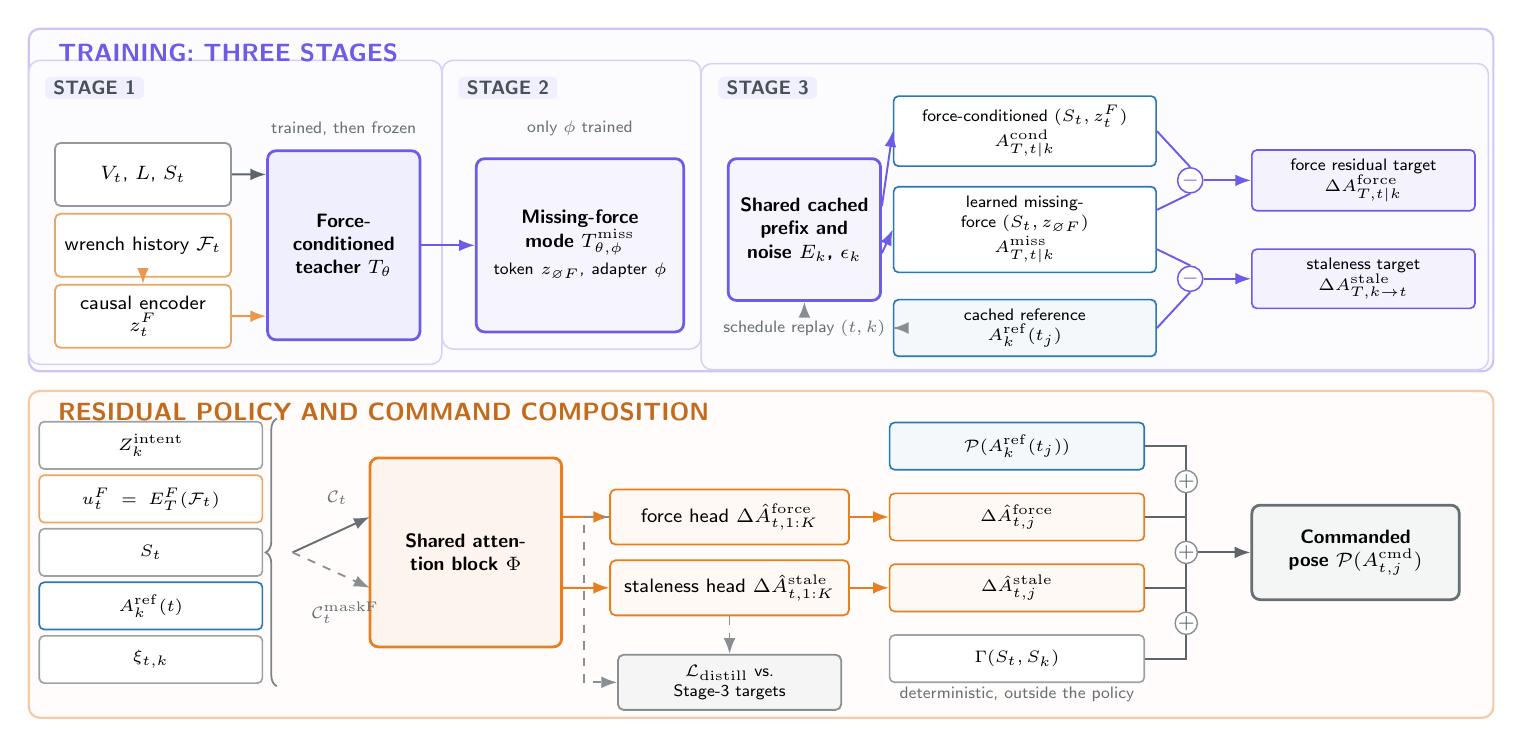
\begin{tikzpicture}[x=1cm,y=1cm]

  \begin{scope}[on background layer]
    \filldraw[rounded corners=4pt,fill=cTeacher!2,draw=cTeacher!35,line width=0.8pt]
      (0,4.40) rectangle (18.6,8.75);
    \filldraw[rounded corners=4pt,fill=cFast!2,draw=cFast!40,line width=0.8pt]
      (0,0) rectangle (18.6,4.15);
  \end{scope}

  % =========================================================== TRAINING PANEL
  \node[ptitle,text=cTeacher,anchor=west] at (0.25,8.45)
    {TRAINING: THREE STAGES};

  % ---- Stage 1: force-conditioned teacher
  \node[stagelab,fill=cTeacher!10,anchor=west] (stage1) at (0.20,8.00) {STAGE 1};
  \node[block] (obs) at (1.45,6.90) {$V_t$,\ $L$,\ $S_t$};
  \node[block,draw=cFast!70] (fh) at (1.45,6.00) {wrench history $\mathcal F_t$};
  \node[block,draw=cFast!70] (enc) at (1.45,5.10) {causal encoder\\$z_t^F$};
  \node[hero,draw=cTeacher,fill=cTeacher!10,text width=17mm,minimum height=24mm]
    (tea) at (4.00,6.00) {Force-conditioned teacher $T_\theta$};
  \node[note] (tag1) at (4.00,7.48) {trained, then frozen};

  \draw[flow] (obs.east) -- ([yshift=9mm]tea.west);
  \draw[flow,draw=cFast!80] (fh.south) -- (enc.north);
  \draw[flow,draw=cFast!80] (enc.east) -- ([yshift=-9mm]tea.west);

  % ---- Stage 2: missing-force mode
  \node[stagelab,fill=cTeacher!10,anchor=west] (stage2) at (5.45,8.00) {STAGE 2};
  \node[hero,draw=cTeacher,fill=cTeacher!6,text width=24mm,minimum height=22mm]
    (miss) at (7.00,6.00)
    {Missing-force mode $T_{\theta,\phi}^{\mathrm{miss}}$\\[1.5pt]
     {\fontsize{6.2}{7.2}\selectfont\mdseries token $z_{\varnothing F}$, adapter $\phi$}};
  \node[note] (tag2) at (7.00,7.48) {only $\phi$ trained};
  \draw[flow,draw=cTeacher] (tea.east) -- (miss.west);

  % ---- Stage 3: cached-context targets, built as two differences
  \node[stagelab,fill=cTeacher!10,anchor=west] (stage3) at (8.75,8.00) {STAGE 3};
  \node[hero,draw=cTeacher,fill=cTeacher!6,text width=17mm,minimum height=18mm]
    (ctx) at (9.85,6.20) {Shared cached prefix and noise $E_k$,\ $\epsilon_k$};
  \node[note] (sched) at (9.85,4.95) {schedule replay $(t,k)$};
  \draw[flow,draw=cInk!55] (sched.north) -- (ctx.south);

  \node[small,draw=cSlow,text width=31mm] (pcond) at (12.65,7.45)
    {force-conditioned $(S_t,z_t^F)$\\$A_{T,t|k}^{\mathrm{cond}}$};
  \node[small,draw=cSlow,text width=31mm] (pmiss) at (12.65,6.20)
    {learned missing-force $(S_t,z_{\varnothing F})$\\$A_{T,t|k}^{\mathrm{miss}}$};
  \node[small,draw=cSlow,fill=cSlow!5,text width=31mm] (pref) at (12.65,4.95)
    {cached reference\\$A_k^{\mathrm{ref}}(t_j)$};
  \node[op] (subF) at (14.75,6.825) {$-$};
  \node[op] (subS) at (14.75,5.575) {$-$};

  \draw[flow,draw=cTeacher] ([yshift=3mm]ctx.east) -- (pcond.west);
  \draw[flow,draw=cTeacher] ([yshift=-3mm]ctx.east) -- (pmiss.west);
  \draw[flow,draw=cInk!55] (sched.east) -- (pref.west);

  \node[small,draw=cTeacher,fill=cTeacher!8,text width=26mm] (tgtF) at (16.95,6.825)
    {force residual target\\$\Delta A_{T,t|k}^{\mathrm{force}}$};
  \node[small,draw=cTeacher,fill=cTeacher!8,text width=26mm] (tgtS) at (16.95,5.575)
    {staleness target\\$\Delta A_{T,k\to t}^{\mathrm{stale}}$};
  \draw[plain,draw=cTeacher] (pcond.east) -- (subF.north);
  \draw[plain,draw=cTeacher] ([yshift=2.5mm]pmiss.east) -- (subF.south);
  \draw[flow,draw=cTeacher] (subF.east) -- (tgtF.west);
  \draw[plain,draw=cTeacher] ([yshift=-2.5mm]pmiss.east) -- (subS.north);
  \draw[plain,draw=cTeacher] (pref.east) -- (subS.south);
  \draw[flow,draw=cTeacher] (subS.east) -- (tgtS.west);

  \begin{scope}[on background layer]
    \node[rounded corners=4pt,fill=cTeacher!2,draw=cTeacher!28,line width=0.55pt,
          inner sep=2mm,fit=(stage1)(obs)(fh)(enc)(tea)(tag1)] {};
    \node[rounded corners=4pt,fill=cTeacher!2,draw=cTeacher!28,line width=0.55pt,
          inner sep=2mm,fit=(stage2)(miss)(tag2)] {};
    \node[rounded corners=4pt,fill=cTeacher!2,draw=cTeacher!28,line width=0.55pt,
          inner sep=1.6mm,fit=(stage3)(ctx)(sched)(pcond)(pref)(tgtF)(tgtS)] {};
  \end{scope}

  % ========================================================= DEPLOYMENT PANEL
  \node[ptitle,text=cFast!85!black,anchor=west] at (0.25,3.88)
    {RESIDUAL POLICY AND COMMAND COMPOSITION};

  % ---- conditioning set of Eq. (14)
  \node[small,text width=26mm] (k1) at (1.55,3.46) {$Z_k^{\mathrm{intent}}$};
  \node[small,draw=cFast!70,text width=26mm] (k2) at (1.55,2.78)
    {$u_t^F=E_T^F(\mathcal F_t)$};
  \node[small,text width=26mm] (k3) at (1.55,2.10) {$S_t$};
  \node[small,draw=cSlow,text width=26mm] (k4) at (1.55,1.42) {$A_k^{\mathrm{ref}}(t)$};
  \node[small,text width=26mm] (k5) at (1.55,0.74) {$\xi_{t,k}$};

  \draw[decorate,decoration={brace,amplitude=4pt,mirror},draw=cInk!60,line width=0.65pt]
    (3.15,3.80) -- (3.15,0.40);
  \coordinate (btip) at (3.35,2.10);

  \node[hero,draw=cFast,fill=cFast!8,text width=22mm,minimum height=24mm]
    (phi) at (5.55,2.10) {Shared attention block $\Phi$};
  \draw[flow,draw=cInk!70] (btip) -- (4.33,2.55);
  \draw[dashflow] (btip) -- (4.33,1.65);
  \node[note,anchor=south] at (3.92,2.58) {$\mathcal C_t$};
  \node[note,anchor=north] at (4.02,1.60) {$\mathcal C_t^{\mathrm{maskF}}$};

  \node[block,draw=cFast,fill=cFast!5,text width=28mm,minimum height=7mm]
    (hF) at (8.90,2.55) {force head $\Delta\hat A^{\mathrm{force}}_{t,1:K}$};
  \node[block,draw=cFast,fill=cFast!5,text width=28mm,minimum height=7mm]
    (hS) at (8.90,1.65) {staleness head $\Delta\hat A^{\mathrm{stale}}_{t,1:K}$};
  \draw[flow,draw=cFast] ([yshift=4.5mm]phi.east) -- (hF.west);
  \draw[flow,draw=cFast] ([yshift=-4.5mm]phi.east) -- (hS.west);

  \node[loss] (ldist) at (8.90,0.45)
    {$\mathcal L_{\mathrm{distill}}$ vs. Stage-3 targets};
  \draw[dashflow] (hS.south) -- (ldist.north);
  \draw[dashflow] (hF.west) -- ++(-0.32,0) |- (ldist.west);

  % ---- composition: one term of Eq. (1) per row
  \node[small,draw=cSlow,fill=cSlow!5,text width=30mm] (c1) at (12.55,3.45)
    {$\mathcal P(A_k^{\mathrm{ref}}(t_j))$};
  \node[small,draw=cFast,fill=cFast!5,text width=30mm] (c2) at (12.55,2.55)
    {$\Delta\hat A^{\mathrm{force}}_{t,j}$};
  \node[small,draw=cFast,fill=cFast!5,text width=30mm] (c3) at (12.55,1.65)
    {$\Delta\hat A^{\mathrm{stale}}_{t,j}$};
  \node[small,text width=30mm] (c4) at (12.55,0.75) {$\Gamma(S_t,S_k)$};
  \node[note] at (12.55,0.30) {deterministic, outside the policy};

  \draw[flow,draw=cFast] (hF.east) -- (c2.west);
  \draw[flow,draw=cFast] (hS.east) -- (c3.west);

  \coordinate (bus) at (14.70,2.10);
  \draw[plain] (c1.east) -- (14.70,3.45) -- (bus);
  \draw[plain] (c4.east) -- (14.70,0.75) -- (bus);
  \draw[plain] (c2.east) -- (14.70,2.55);
  \draw[plain] (c3.east) -- (14.70,1.65);

  \node[hero,draw=cInk!70,fill=cInk!5,text width=24mm,minimum height=12mm]
    (cmd) at (16.85,2.10) {Commanded pose $\mathcal P(A^{\mathrm{cmd}}_{t,j})$};
  \draw[flow] (bus) -- (cmd.west);
  \node[opf] at (14.70,3.00) {$+$};
  \node[opf] at (14.70,2.10) {$+$};
  \node[opf] at (14.70,1.20) {$+$};

\end{tikzpicture}
\end{document}
